\section{Conclusions and Outlook}\label{conclusion_section}

This note has discussed the multiple coulomb scattering technique for estimating the momentum of a three dimensional reconstructed track and has provided motivation for demonstration of the capabilities of this tool within the neutrino LArTPC community. This technique will be important for future cross section and oscillation measurements from the {\ub} collaboration. The details of the implementation of this code have been described. The gaussian nature of scatters predicted by the Highland formula has been demonstrated. The performance of this method has been quantified in two different forms of simulation of fully contained tracks (truth-selected simulated BNB neutrino events with {\sc MCTracks} and reconstructed tracks, and automatically-selected selected BNB + cosmic neutrino events) as well as in approximately 0.5e20 POT of {\ub} data. Additionally, the performance of this method on exiting tracks in simulation has been quantified.\\

To summarize the performance on the different fully contained track samples, the bias and resolution for the different samples are overlaid in Figure \ref{MCS_range_bias_resolution_masteroverlay_fig}. In general, performance on reconstructed tracks in MC and data agree though extremely limited statistics above 1 GeV range-based momentum makes more concrete statements difficult. The energy resolution with reconstructed tracks tends to be slightly worse than that with {\sc MCTracks} which can be attributed to imperfect track reconstruction and other detector effects to which {\sc MCTracks} are insensitive like broken wires and simulated noise. No samples have a fractional bias above 5\%.\\

Other uses besides momentum reconstruction for the MCS technique have been described, including using it as a tool for identification of poorly reconstructed tracks and particle identification. In the appendices can be found descriptions of the methods used to optimize the segment length (14 cm) and detector resolution term (3 mrad) in the MCS algorithm, as well as studies of using MCS to determine track direction, and studies to justify using inverse momentum to compute bias and resolution metrics.\\

This note is by no means a complete, end-all analysis of the MCS code; there are many useful ways to continue this study.\\

Additional avenues to further this analysis include:
\begin{itemize}
	\item Determining the impact that spacecharge (electric field nonuniformities most significant near the edges of the TPC) has on the MCS algorith. This study should likely be prioritized!
	\item Determining if the MCS algorithm can be used for muon/pion discrimination (pions should have more larger-angle hard scatters than muons).
	\item Quantifying the performance of the MCS algorithm as a function of track angle (which is briefly explored in Appendix \ref{AngleStudy_MCBNBRecoTrack_section}).
	\item Using calorimetry to determine energy loss upstream of a segment rather than assuming average MIP deposited energy or using an integral of the PDG stopping power curve... this will be best especially for cases where large amounts of energy is lost to delta rays.
	\item Using a likelihood map (plot of likelihood vs. step in raster scan) to assign an uncertainty to the returned MCS momentum value (maybe something like the magnitude of the second derivative?)
\end{itemize}


\begin{figure}
\centering
\mbox{
	\subfigure[\textit{MCS momentum bias as a function of range momentum. The vertical error bars are computed as $\frac{\sigma_{fit}}{\sqrt{N}}$, and the horizontal error bars indicate bin width.}]
	{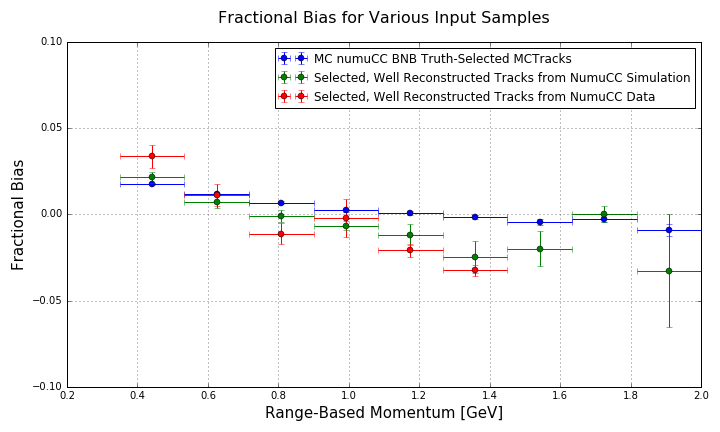
\includegraphics[width=80mm]{Figures/MCS_range_bias_multiplesamples.png}}
	\quad
	\subfigure[\textit{MCS momentum resolution as a function of range momentum. The vertical error bars are computed as $\frac{\sigma_{fit}}{\sqrt{2N}}$, and the horizontal error bars indicate bin width.}]
	{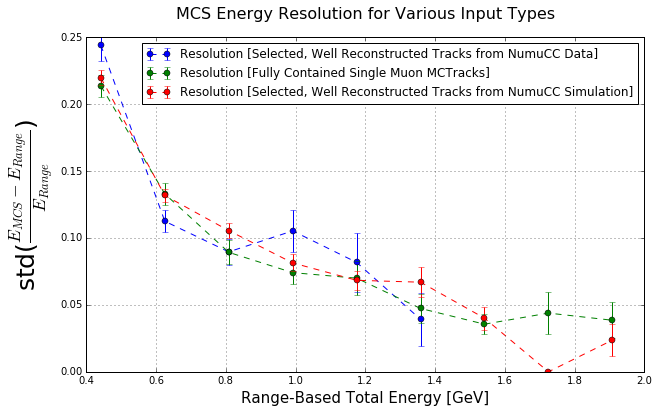
\includegraphics[width=80mm]{Figures/MCS_range_resolution_multiplesamples.png}}
	}
\caption{\textit{MCS momentum resolution for simulated truth-selected BNB numuCC {\sc MCTracks} discussed in Section \ref{MCBNBMCTrack_performance_section} (blue), automatically selected contained numuCC-induced muons from simulated BNB+cosmics where the track is well-reconstructed and matches with the true muon track discussed in Section \ref{MC_performance_section} (green), and automatically selected contained numuCC-induced muons from MicroBooNE data where the track is deemed well-reconstructed and likely-muon from hand scanning discussed in Section \ref{data_performance_section}.}}
\label{MCS_range_bias_resolution_masteroverlay_fig}
\end{figure}











\clearpage
\section{Possible Plots for Publication}\label{publicplots_section}
This section includes plots that to be considered for the publication. The publication should have its scope kept small so as to get it published in a very quick time scale. These plots of course can be modified, their captions changed, etc... I am just putting them here to paint a picture for the readers of this technote what I think should be included in the publication.
\begin{enumerate}
	\item Figure \ref{pub_plot_1} is a general image whose purpose is to aid the reader in understanding what MCS is and how the code works. I'm not sure this one is public-domain, but I can easily make my own version of it if necessary.
	\item Figure \ref{pub_plot_2} is an image whose purpose is to validate using range-based momentum in place of true-momentum when the analysis is done on real data where true-momentum obviously is unknown.
	\item Figure \ref{pub_plot_3} is an image whose purpose is to show that the segment-to-segment angular scatters are indeed gaussian as predicted by the Highland formula, and therefore the basis for this technique is sound.
	\item Figure \ref{pub_plot_4} is an image showing the MCS momentum versus range momentum for the automatically selected, handscanned data events.
	\item Figure \ref{pub_plot_5} is an overlay of MCS momentum bias and resolution for directly comparable samples in data and MC. The {\sc MCTrack} sample is left out of this plot because {\sc MCTracks} are very {\ub} specific. Also the x-axis cuts off at around 1.3 GeV as statistics become very limited after that.
	\item Figure \ref{pub_plot_6} is the MCS bias and resolution for the sample of \textit{exiting} reconstructed tracks.
\end{enumerate}

% Image describing MCS idea
\begin{figure}[ht!]
\centering
	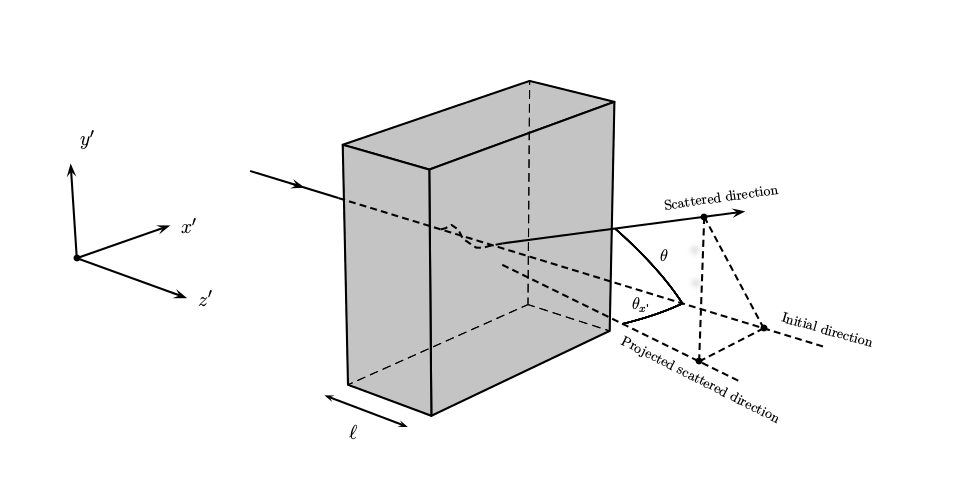
\includegraphics[width=0.5\linewidth]{Figures/static_figs/mcs_nocap.png} \\
\caption{\textit{The particle's trajectory is deflected as it traverses through the material \cite{leonidas1}.}}\label{pub_plot_1}
\end{figure}

% Image validating range-based energy
\begin{figure}
\centering
\mbox{
	\subfigure[\textit{Range energy bias as a function of true energy.}]
	{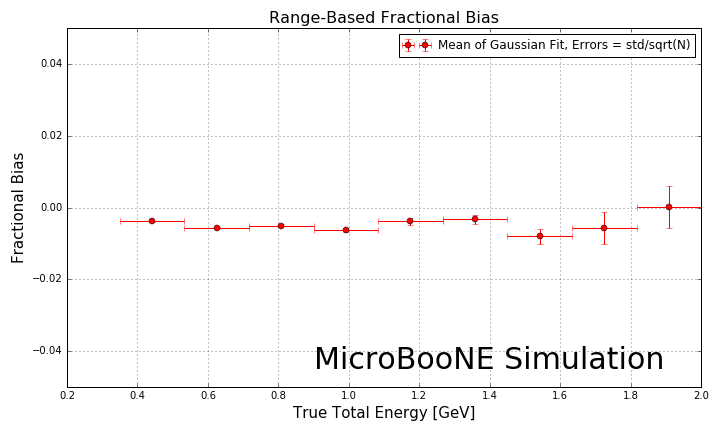
\includegraphics[width=75mm]{Figures/true_range_bias_MCBNBMCTrack.png}}
	\quad
	\subfigure[\textit{Range energy resolution as a function of true energy.}]
	{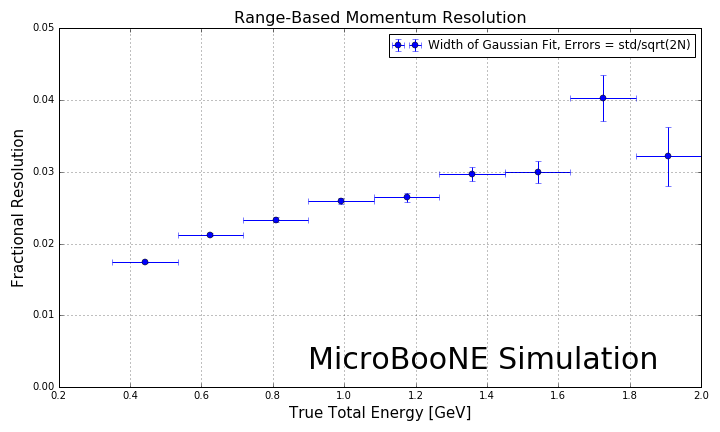
\includegraphics[width=75mm]{Figures/true_range_resolution_MCBNBMCTrack.png}}
	}
\caption{\textit{Range energy and true energy bias and resolution for the {\sc MCTrack} sample described in Section \ref{MCBNBMCTrack_eventselection_section}.}}
\label{pub_plot_2}
\end{figure}

% Highland validation image
\begin{figure}
\centering
	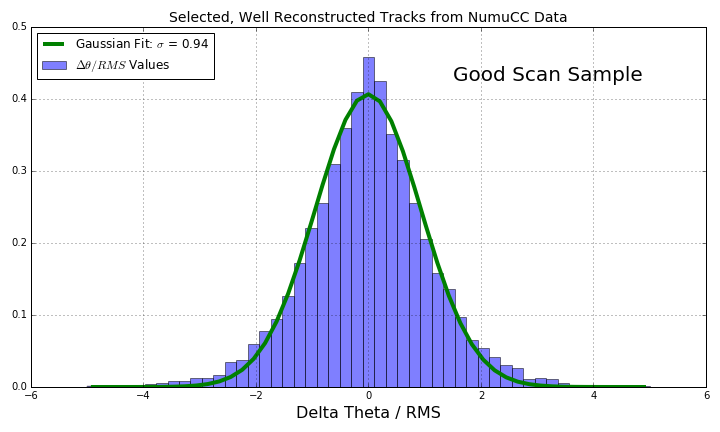
\includegraphics[width=75mm]{Figures/Highland_validation_DataBNBSelectedRecoTrack_goodscan.png}
\caption{\textit{10 cm segment angular deviations divided by expected Highland RMS for the sample of well reconstructed (as determined by the hand scanning), neutrino induced muons in {\ub}.}}
\label{pub_plot_3}
\end{figure}


% Image showing MCS momentum vs range momentum the handscanned data events
\begin{figure}
\centering
	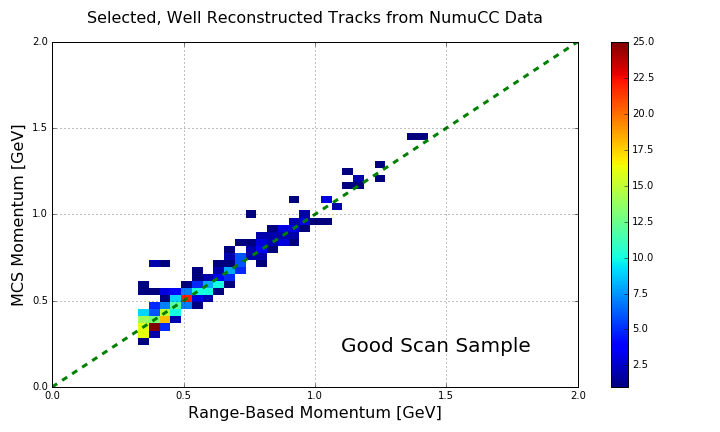
\includegraphics[width=75mm]{Figures/MCS_range_momentum_DataRecoTracks_goodhandscan.png}
\caption{\textit{MCS computed momentum versus range momentum for the selected neutrino-induced fully contained muon sample in data hand-scanned as having well reconstructed, likely-muon tracks.}}
\label{pub_plot_4}
\end{figure}


% Image showing bias and resolution for single mu MCTracks, auto selected neutrino in MC (truth muon only), auto selected neutrino in data (with handscan)

\begin{figure}
\centering
\mbox{
	\subfigure[\textit{MCS energy bias as a function of range energy.}]
	{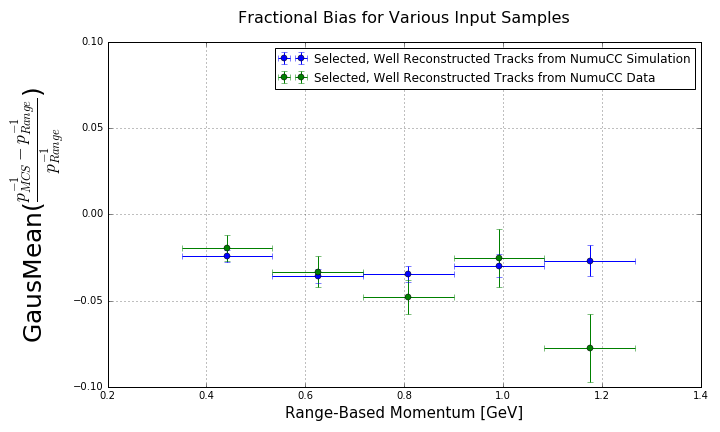
\includegraphics[width=80mm]{Figures/MCS_range_bias_multiplesamples_publicplot.png}}
	\quad
	\subfigure[\textit{MCS energy resolution as a function of range energy.}]
	{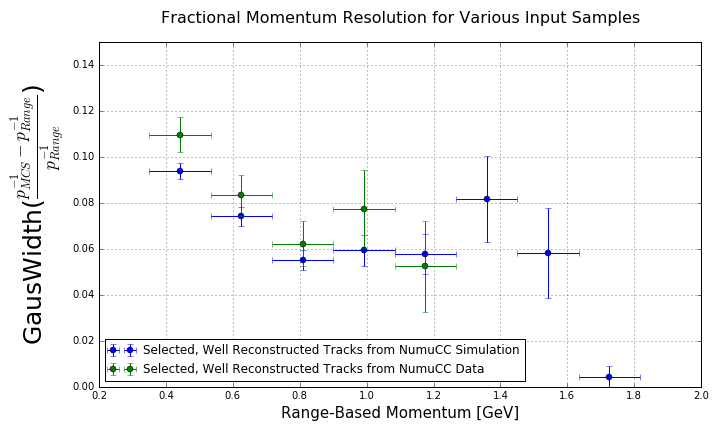
\includegraphics[width=80mm]{Figures/MCS_range_resolution_multiplesamples_publicplot.png}}
	}
\caption{\textit{MCS momentum resolution for automatically selected contained numuCC-induced muons from simulated BNB+cosmics where the track is well-reconstructed and matches with the true muon track discussed in Section \ref{MC_performance_section} (blue), and automatically selected contained numuCC-induced muons from MicroBooNE data where the track is deemed well-reconstructed and likely-muon from hand scanning discussed in Section \ref{data_performance_section} (green).}}\label{pub_plot_5}
\end{figure}



\begin{figure}
\centering
\mbox{
	\subfigure[\textit{MCS momentum bias. The vertical error bars are computed as $\frac{\sigma_{fit}}{\sqrt{N}}$, and the horizontal error bars indicate bin width.}]
	{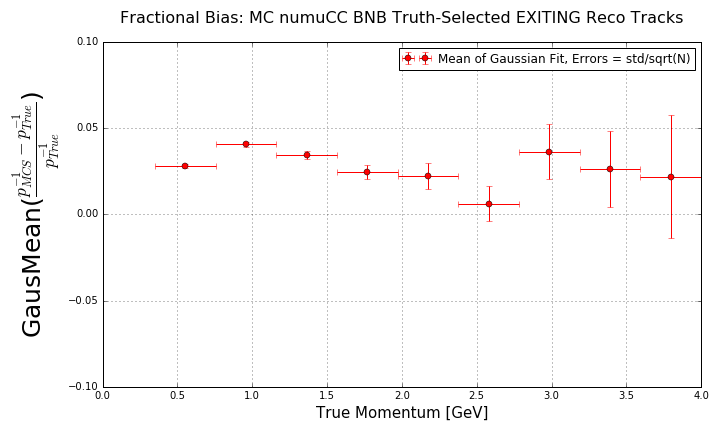
\includegraphics[width=75mm]{Figures/MCS_true_exiting_bias_MCBNBRecoTrackExiting.png}}
	\quad
	\subfigure[\textit{MCS momentum resolution. The vertical error bars are computed as $\frac{\sigma_{fit}}{\sqrt{2N}}$, and the horizontal error bars indicate bin width.}]
	{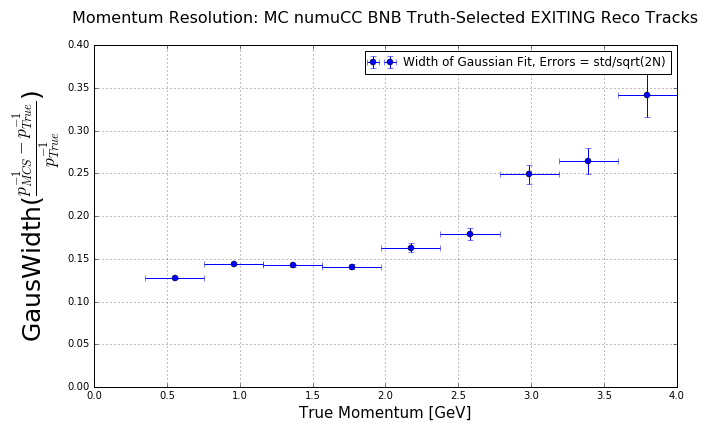
\includegraphics[width=75mm]{Figures/MCS_true_exiting_resolution_MCBNBRecoTrackExiting.png}}
	}
\caption{\textit{MCS momentum bias as a function of true momentum for this sample of exiting muon reconstructed tracks. The vertical error bars are computed as $\frac{\sigma_{fit}}{\sqrt{N}}$, and the horizontal error bars indicate bin width.}}\label{pub_plot_6}
\end{figure}
